\chapter{An algorithm for testing pattern-avoidance of a special pattern}
\label{chap:walking}
In the previous chapter, we have seen an algorithm for a general forbidden pattern. In this chapter, we introduce a special kind of a pattern, satisfying additional conditions, for which we can produce a much faster algorithm.

\section{Walking pattern}
\begin{defn}
A \emph{walk} in a matrix $P$ is a sequence of some of its entries, beginning in the top left corner and ending in the bottom right one. If an entry at the position $[i,j]$ is in the sequence, the next one is either $[i+1,j]$ or $[i,j+1]$. Let $w$ denote the width of $P$ and $h$ denote its height, the length of an arbitrary walk is equal to $w+h-1$ and we denote elements of the sequence by $w_1,w_2,\cdots,w_{w+h-1}$.
\end{defn}
\begin{defn}
We call a binary matrix $P$ a \emph{walking pattern} if there is a walk in $P$ such that all the one-entries of $P$ are contained on the walk.
\end{defn}
\begin{figure}[h!]
\centering
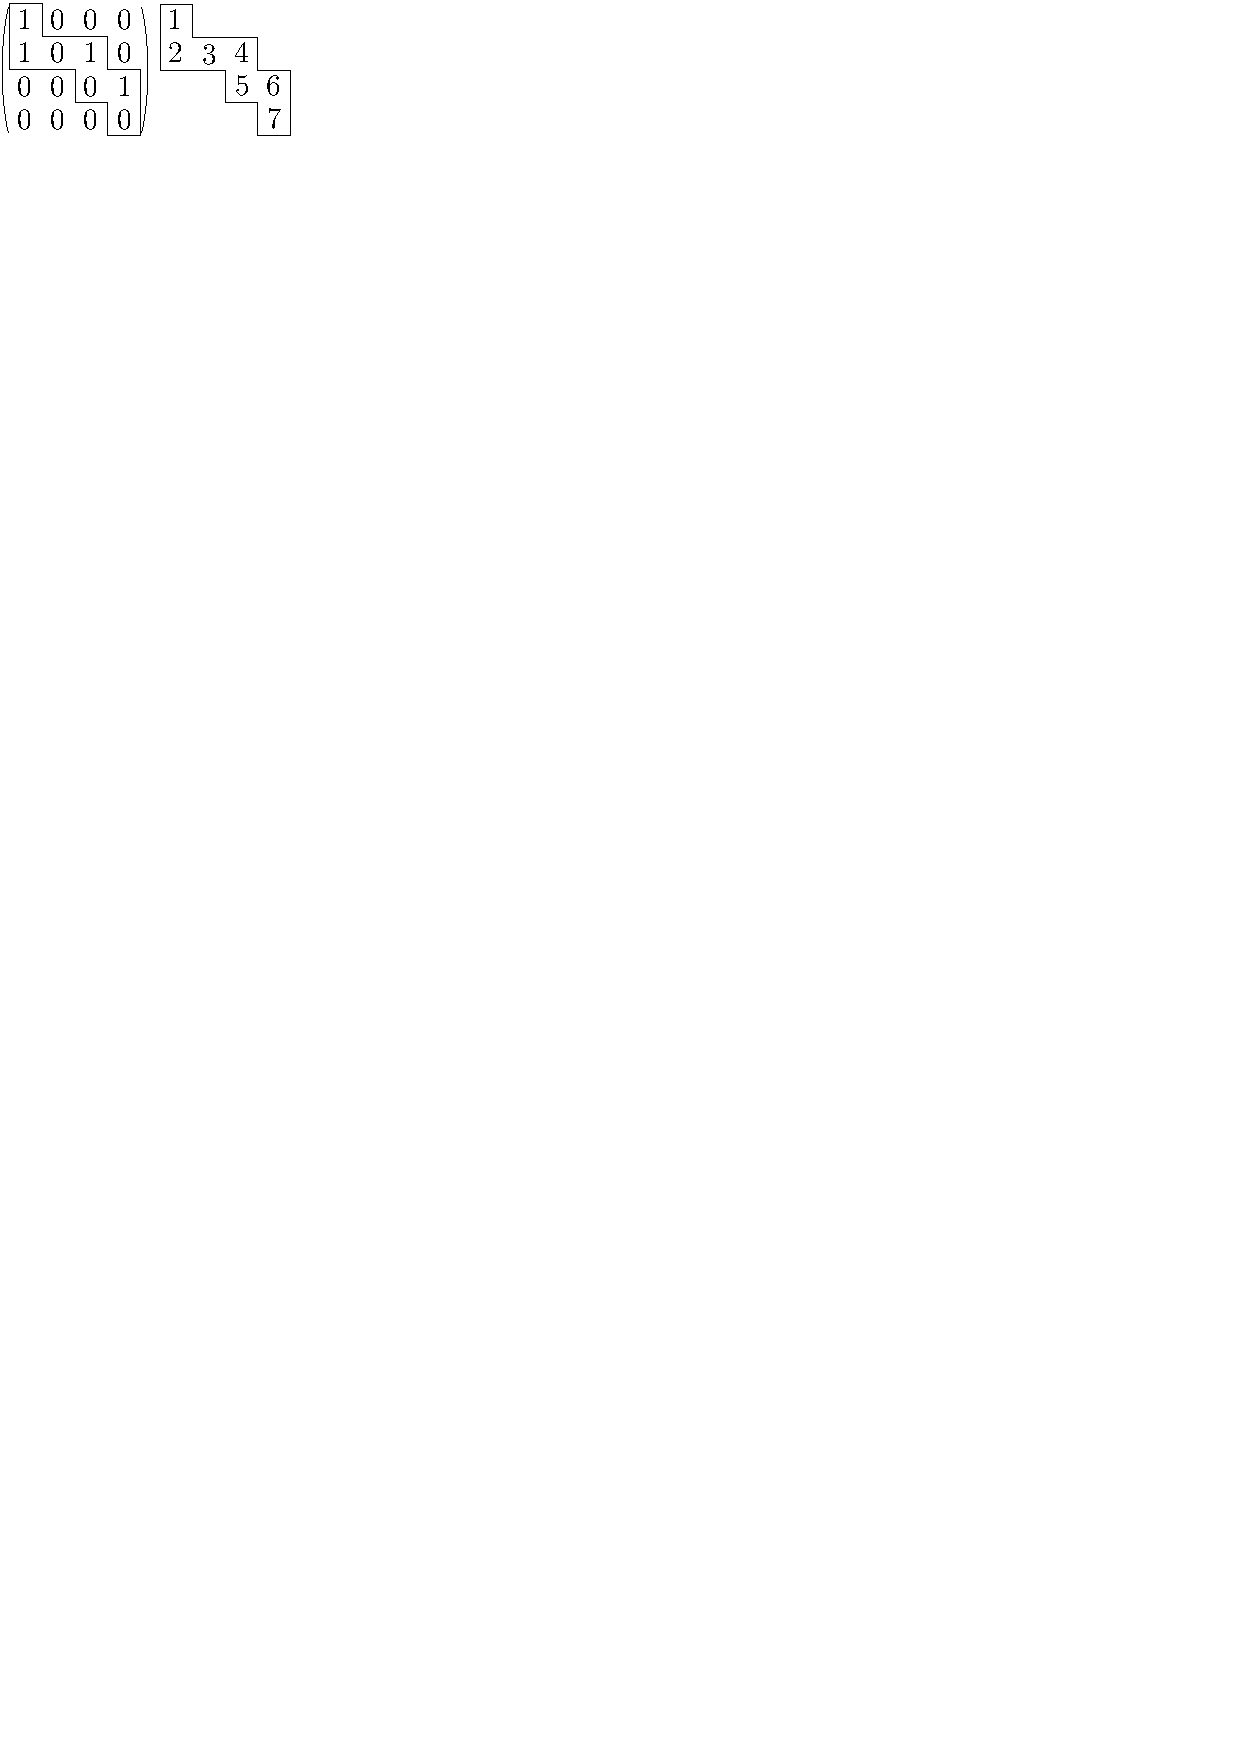
\includegraphics[width=90mm]{../img/walk.pdf}
\caption{An example of a walk $W$ in matrix $M$ and the order of entries in $W$.}
\label{walk}
\end{figure}

In Figure \ref{walk} the matrix $M$ is a walking pattern as all the one-entries are included in a walk. We can also see that not all entries of a walk need to be one-entries.

It can be shown a walking pattern is exactly a matrix avoiding a forbidden pattern $\left(\begin{smallmatrix}
0 & 1 \\
1 & 0
\end{smallmatrix}\right)$.

\section{Dynamic program}
Next, we show an algorithm deciding whether a walking pattern $P$ is contained in a big matrix $M$ or not.

The pattern $P$ is a walking pattern, so there is a walk containing all the one-entries of $P$. We choose one such walk arbitrarily. For each entry of the walk we remember whether its value in $P$ is one or zero and whether the walk continues from the entry vertically, in which case we call it a \emph{vertical entry} or horizontally, calling it a \emph{horizontal entry}. The last entry is an exception and it is neither horizontal nor vertical.
\begin{defn}
For an element $e$ of $M$ at the position $[i,j]$ ($[0,0]$ is the first element), the matrix $M_{\leq e}$ is a $(i+1)\times(j+1)$ submatrix of $M$ consisting of rows with the index smaller than or equal to $i$ and columns with the index smaller than or equal to $j$. The element $e$ then lies in the bottom right corner.
\end{defn}
To determine whether $P$ is contained in $M$ we find out for each element $e$ of $M$ what is the biggest index $k$ such that there exists a mapping of $P_{\leq w_k}$ to $M_{\leq e}$. If there is an element for which we manage to find the whole pattern ($k=w+h-1$), $P$ is contained in $M$; otherwise, it is avoided.

\subsection{Inner structures}
The algorithm uses two structures. For each $w_k$ we remember whether it is a one-entry or zero-entry in $P$ and whether it is a vertical entry or horizontal entry.

The second structure is a matrix of the same size as $M$. For each element $e$ at the position $[i,j]$ we store two numbers. The number $c_v(e)$ is the biggest index $k$ such that $w_k$ is a vertical entry and there is a mapping of $P_{\leq w_k}$ to $M_{\leq e}$, in which $w_k$ is being mapped to the $j$-th column. The number $c_h(e)$, symmetrically, is the biggest index $k$ such that $w_k$ is a horizontal entry and there is a mapping of $P_{\leq w_k}$ to $M_{\leq e}$, in which $w_k$ is being mapped to the $i$-th row.

\subsection{The algorithm}
\begin{defn}
A \emph{diagonal} of the matrix $M$ is a subset of elements of $M$, such that all elements have the same sum of their coordinates.
\end{defn}
For example, the zero diagonal only consists of the element $[0,0]$, the first diagonal contains elements $[0,1]$ and $[1,0]$, and so on.
\begin{figure}[h!]
\centering
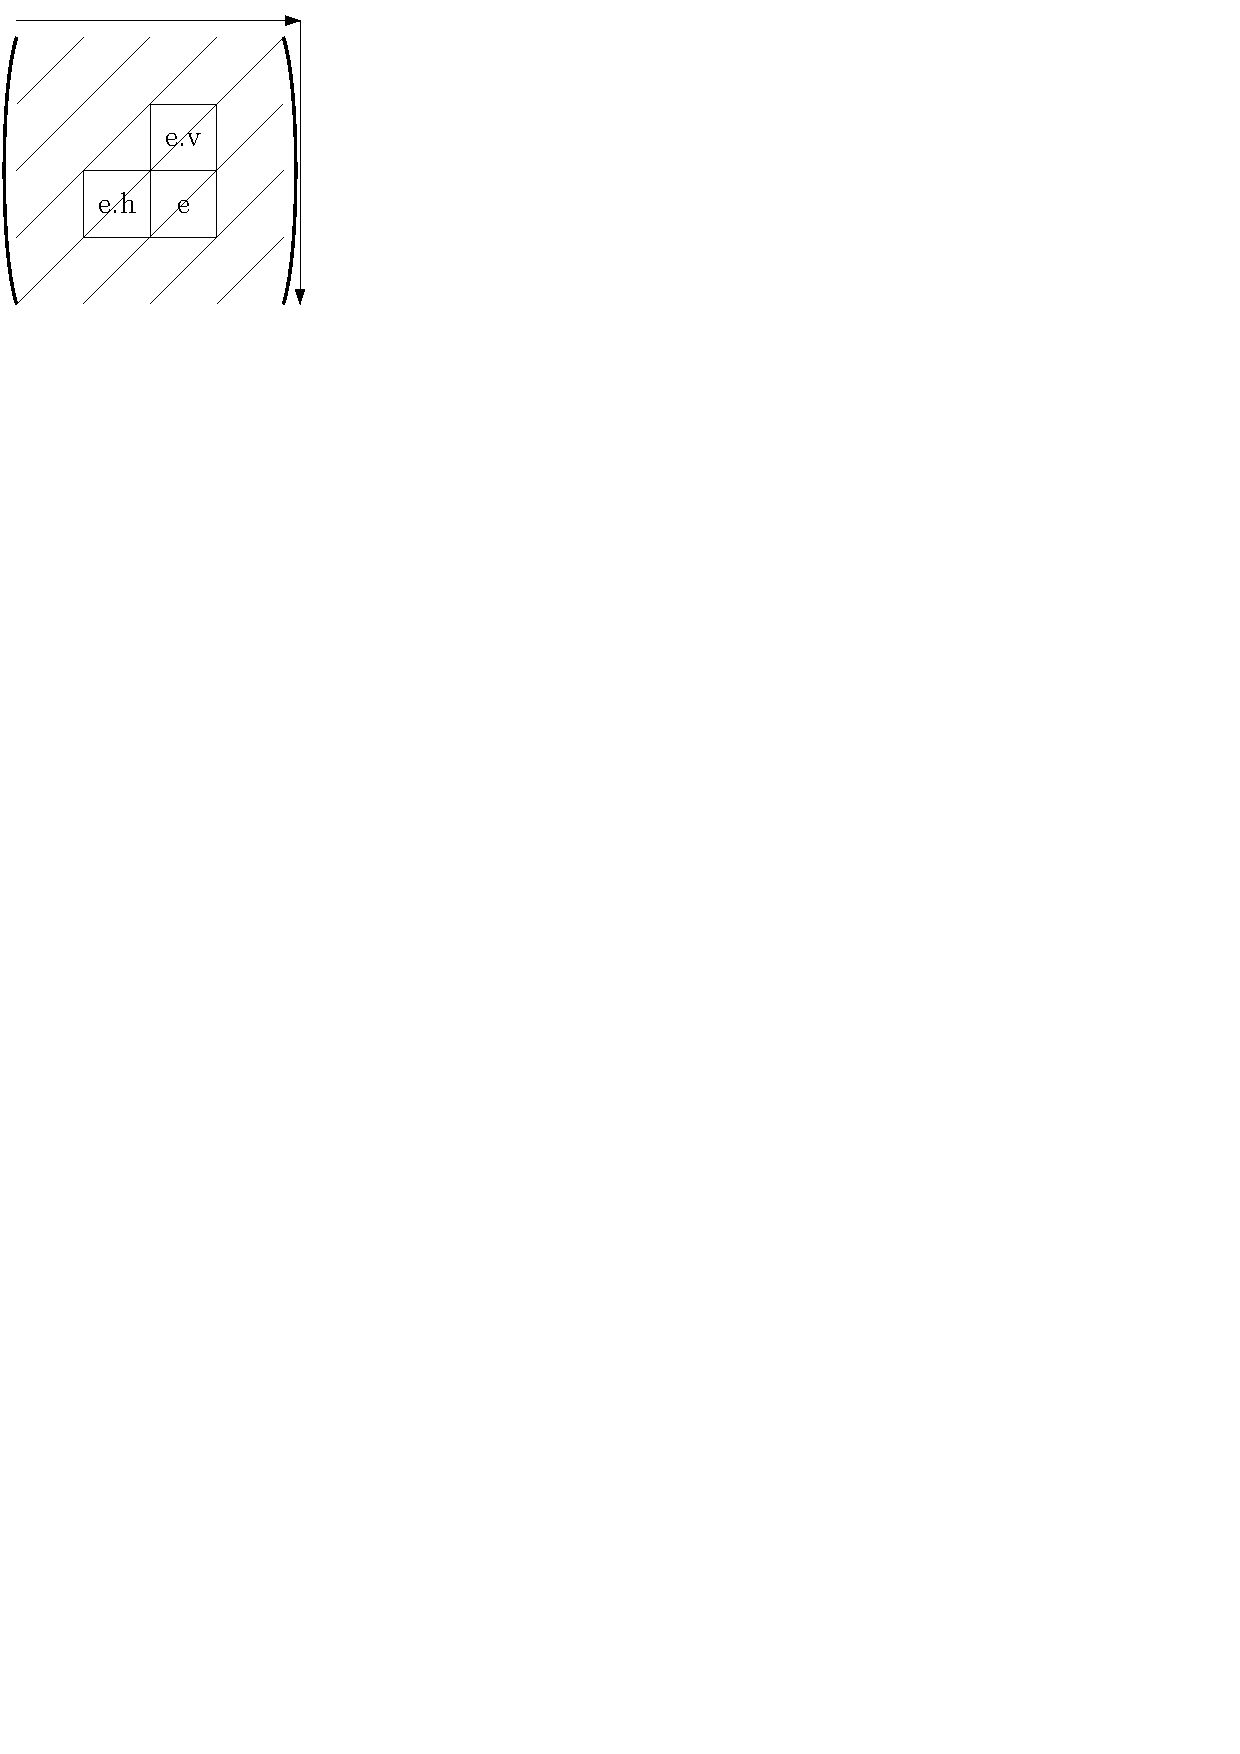
\includegraphics[width=60mm]{../img/walking_alg.pdf}
\caption{Diagonals of an matrix and the order in which the algorithm for walking pattern iterates through them.}
\end{figure}

The algorithm iterates through diagonals. For simplicity, in the pseudo-code below we do not deal with elements outside $M$ (like $[-1,0]$) explicitly. Instead, for those elements, we assume $c_v=c_h=0$. When we ask whether $w_k$ can be mapped to $e$, where $e$ is an element of $M$, we check whether $w_k$ stands for a one-entry of $P$ and if it does, we require $e$ to be a one-entry too.

For an $n\times n$ matrix $M$ the algorithm works as follows:
\begin{enumerate}
\item For $d=0,\cdots,2n-2$
\item \hspace{5mm} For $e$ element of $d$-th diagonal at the position $[i,j]$
\item \hspace{1cm} $e_v:=[i-1,j]$
\item \hspace{1cm} $e_h:=[i,j-1]$
\item \hspace{1cm} $c_v(e):=c_v(e_v)$
\item \hspace{1cm} $c_h(e):=c_h(e_h)$
\item \hspace{1cm} If $w_{c_v(e_v)+1}$ can be mapped to $e$
\item \hspace{15mm} If $c_v(e_v)+1=w+h-1$
\item \hspace{2cm} Terminate - $M$ contains $P$ as a submatrix
\item \hspace{15mm} If $w_{c_v(e_v)+1}$ is a vertical entry
\item \hspace{2cm} $c_v(e):=c_v(e_v)+1$
\item \hspace{15mm} Else
\item \hspace{2cm} $c_h(e):=max\{c_h(e),c_v(e_v)+1\}$
\item \hspace{1cm} If $w_{c_h(e_h)+1}$ can be mapped to $e$
\item \hspace{15mm} If $c_h(e_h)+1=w+h-1$
\item \hspace{2cm} Terminate - $M$ contains $P$ as a submatrix
\item \hspace{15mm} If $w_{c_h(e_h)+1}$ is a vertical entry
\item \hspace{2cm} $c_v(e):=max\{c_v(e),c_h(e_h)+1\}$
\item \hspace{15mm} Else
\item \hspace{2cm} $c_h(e):=max\{c_h(e),c_h(e_h)+1\}$
\end{enumerate}

\subsection{Correctness}
The first observation we make is that for every element $e$ of $M$ and any element $e'$ above $e$ in the same column $c_v(e')\leq c_v(e)$. This holds because whenever we manage to map $P_{\leq w_k}$ to $M_{\leq e'}$, then the same mapping maps $P_{\leq w_k}$ to $M_{\leq e}$. Similarly, it also holds for every $e$ element of $M$ and any element $e'$ to the left of $e$ in the same row that $c_h(e')\leq c_h(e)$.

The function can terminate before recomputing all elements and we have no guarantee about the state of elements that have not been recomputed. If the function finds the pattern ending in entry $e$, it stops computing at that point, but to prove correctness it is enough to prove the values are correct in $M_{\leq e}$, which has been fully recomputed. If, on the other hand, the function does not find the pattern, it recomputes the whole structure.

We need to show that the values of $c_v$ and $c_h$ are always correct for the recomputed elements at the end of the function. We proceed by induction on diagonals.

For the first diagonal it is definitely true since only $w_1$ can be mapped there and we check that on lines 7 and 14.

When we are recomputing the values of $c_v(e)$ and $c_h(e)$ of an element $e$ in the diagonal $d$, by induction hypothesis, all elements in diagonals $d'<d$ are correctly recomputed. Let $cor$ denote the correct value of $c_v(e)$ as it is defined and $com$ be the computed value. We need to show $cor=com$.

We can already see $cor\geq com$ because it holds after setting $c_v(e)$ on line 5 and we only increase it, if we manage to find an extension of a mapping, in which case there really is a mapping; therefore, $cor$ is greater or equal to the updated value.

To prove $cor\leq com$ we proceed by contradiction. Let us assume $cor>com$. It means there is a mapping of $P_{\leq w_{cor}}$ to $M_{\leq e}$ we have never found. Every such mapping has to map $w_{cor}$ to $e$, because if it did not, the mapping would be possible even for diagonal $d-1$, which is recomputed correctly and the value $cor$ would be copied to $com$ on line 5. Let us assume that $w_{cor-1}$ is a vertical entry (else we proceed analogously). If $P_{\leq w_{cor}}$ can be mapped to $M_{\leq e}$ and $w_{cor-1}$ is a vertical entry, then $P_{\leq w_{cor-1}}$ can be mapped to $M_{\leq e_v}$ and $w_{cor-1}$ must be mapped to the same column as $e$. That means that $c_v(e_v)\geq cor-1$. If $c_v(e_v)=cor-1$ and from knowing $w_{cor}$ can be mapped to $e$, $com\geq c_v(e)\geq c_v(e_v)+1=cor$ because of line 11. Otherwise $c_v(e_v)>cor-1$, but then even from line 5 we get $com\geq cor$, resulting in contradiction.

To prove $c_h(e)$ has the correct value, we proceed symmetrically.

\subsection{Generalization}
The algorithm, with a few minor changes, can also be used for a pattern where all one-entries are contained on a walk from the top right corner to the bottom left one. The program supports both rotations of a walk and when walking pattern is chosen it automatically decides which variant to use.

On the other hand, a direct generalization for a general pattern does not work. While we can index all entries of the pattern, when trying to map a certain $w_k$ to an element $e$ of $M$, it is not sufficient to only check whether $w_l$ is above and $w_l'$ to the left from $e$.
\begin{figure}[h!]
\centering
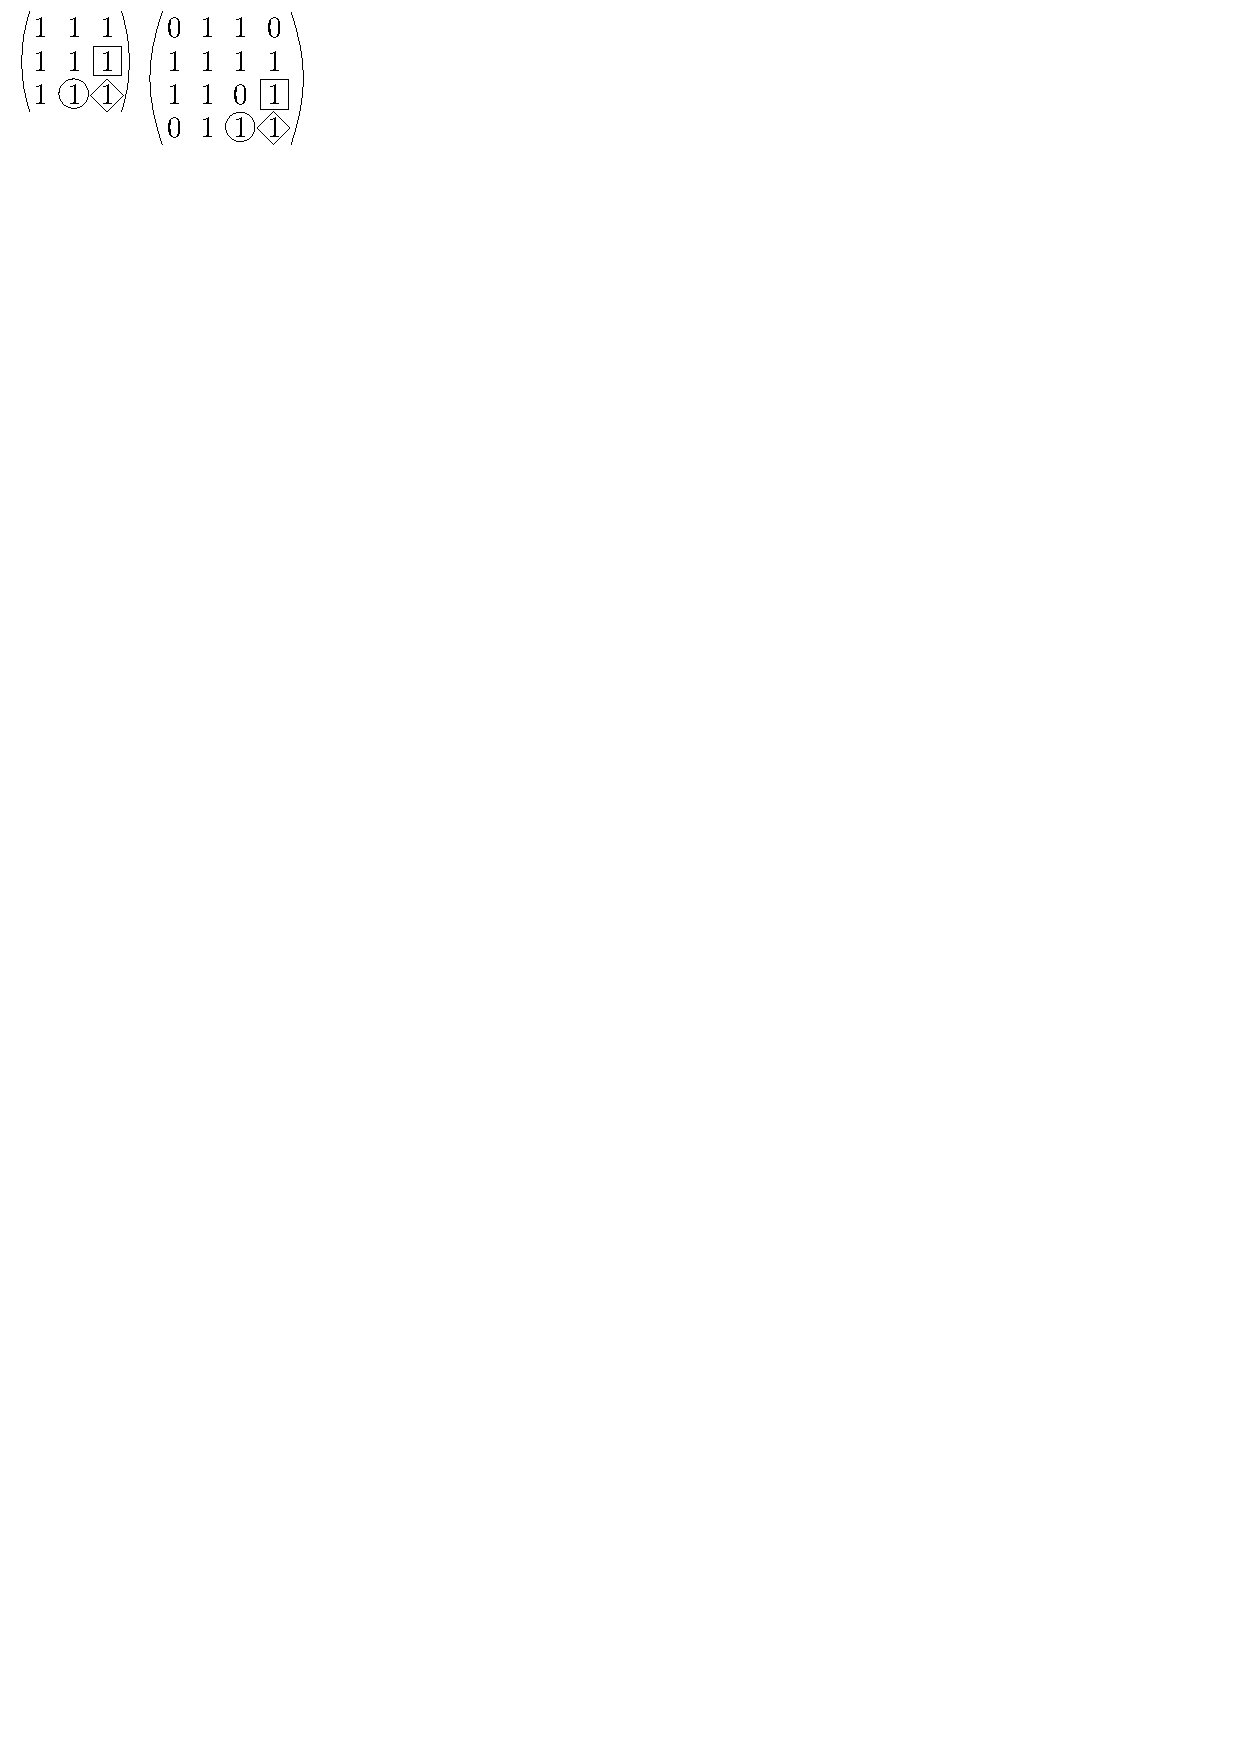
\includegraphics[width=80mm]{../img/nogeneral.pdf}
\caption{The algorithm testing avoidance for walking patterns cannot be easily generalized for all patterns.}
\label{nogeneral}
\end{figure}

In Figure \ref{nogeneral}, the entry of $P$ in the square can be mapped to the element of $M$ in the square and the same holds for entries in the circle but it is not a sufficient condition for the entry of $P$ in the kite to be mapped to the element of $M$ in the kite.